\documentclass{article}
% \usepackage[T1]{fontenc}
% \usepackage[latin9]{inputenc}
\usepackage[top = 2cm, left = 2.5cm, right = 2.5cm, bottom = 2cm]{geometry}
\usepackage{enumitem}
% \usepackage{fontspec}
\usepackage{amsmath}
\usepackage{amsfonts}
\usepackage{hyperref}
\usepackage{amstext}
\usepackage{mdframed}
\usepackage{graphicx}
\usepackage{wrapfig}
\usepackage{caption}
\usepackage{multicol}
\usepackage{mathtools}
\DeclarePairedDelimiter\bra{\langle}{\rvert}
\DeclarePairedDelimiter\ket{\lvert}{\rangle}
\DeclarePairedDelimiterX\braket[2]{\langle}{\rangle}{#1\,\delimsize\vert\,\mathopen{}#2}

\newtheorem{theorem}{Theorem}[section] % This numbers theorems by section
\newtheorem{definition}[theorem]{Definition}
\newtheorem{lemma}[theorem]{Lemma}
\newtheorem{corollary}[theorem]{Corollary}
% \usepackage{bbm}
\makeatletter
\@ifundefined{date}{}{\date{}}
\usepackage{tikz}
\usetikzlibrary{quotes, angles, decorations.markings, intersections}
\usetikzlibrary{calc,patterns,angles,quotes, 3d, intersections, positioning, shapes, automata, positioning}
\usepackage{wasysym}
\makeatother
\usepackage{babel}
\usepackage{color}
\usepackage{graphicx}
\usepackage{hyperref}
\hypersetup{
	colorlinks,
	citecolor=black,
	filecolor=black,
	linkcolor=black,
	urlcolor=black
}


\newcommand{\tbox}[2]{\noindent\fbox{\parbox{\textwidth}{#2}}}

\setlength{\parindent}{0pt}
\begin{document}

\noindent\tbox{01}{
\begin{center}
  \huge Week 2 Assignment
\end{center}
}
    \section*{Question 1}
      \begin{figure}[ht]
        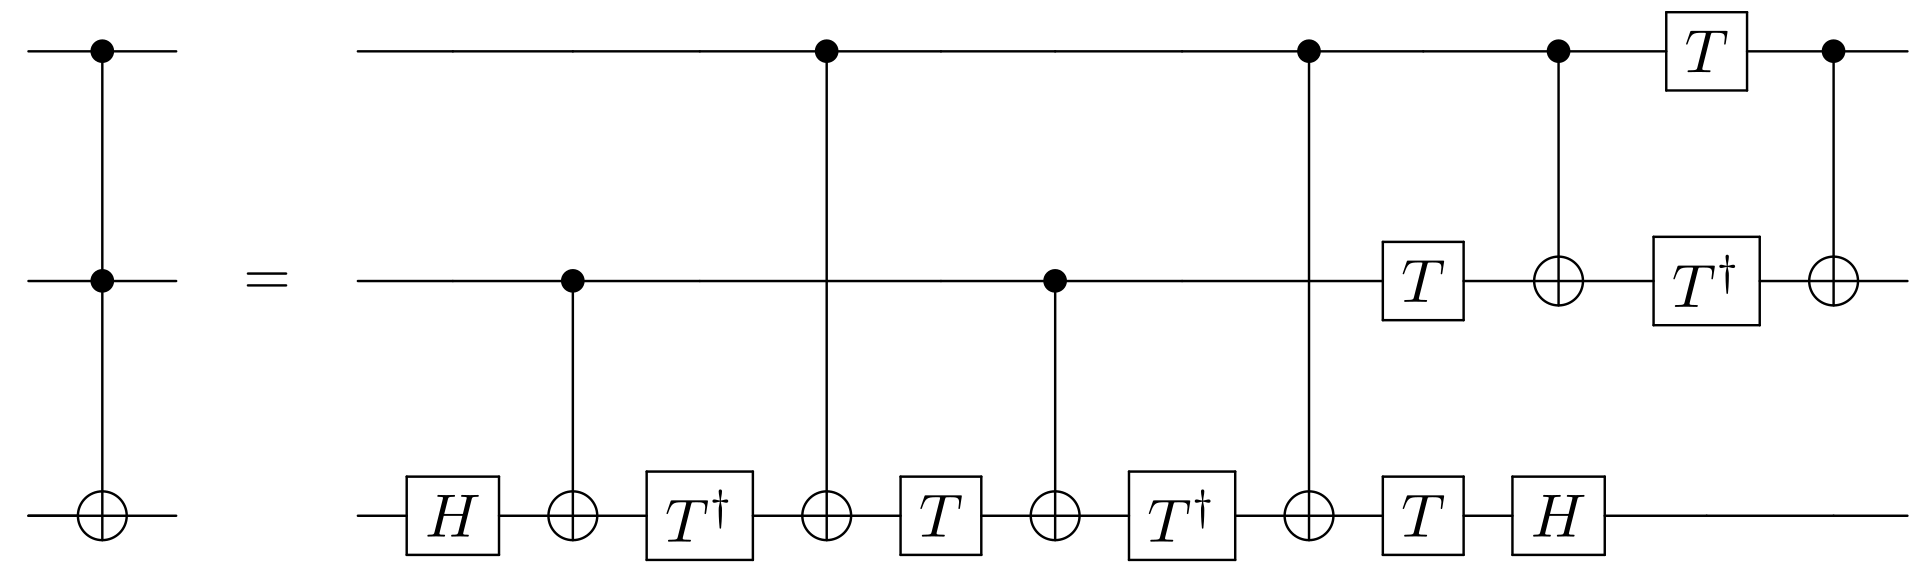
\includegraphics[width=1\textwidth]{q1.png}      
          \centering   
      \end{figure}
      Here, the T gate is also called as $\pi/8$ gate.
      \begin{align*}
        H &= \frac{1}{\sqrt{2}} \begin{pmatrix}
          1 & 1 \\
          1 & -1
          \end{pmatrix} \\
          T &= \begin{pmatrix}
            1 & 0 \\
            0 & e^{i\pi/4}
            \end{pmatrix}
      \end{align*}
    \section*{Question 2}
      \begin{figure}[ht]
        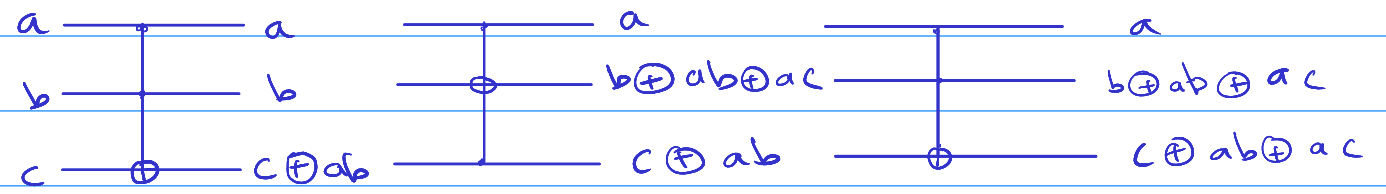
\includegraphics[width=1\textwidth]{q2.png}      
          \centering   
      \end{figure}
      So the idea is that, we need to interconvert $\ket*{110}$ to $\ket*{101}$ and return the same of others. In the shown above diagram, after the first step, the quibits are as shown. In the second step, the second quibit converts as the following:-
      \begin{align*}
        b \oplus ((a).(c \oplus ab)) &= b \oplus ((ac \oplus a.ab)) \\
        &= b \oplus ((ac \oplus ab)) \\
        &= b \oplus ab \oplus ac \\
      \end{align*}
      In the third step, third quibit becomes the following:-
      \begin{align*}
        (c \oplus ab) \oplus ((a).(b \oplus ab \oplus ac)) &= (c \oplus ab) \oplus (ab \oplus a.ab \oplus a.ac) \\
        &= (c \oplus ab) \oplus (ab \oplus ab \oplus ac) \\
        &= c \oplus ab \oplus ab \oplus ab \oplus ac \\
        &= c \oplus ab \oplus (ab \oplus ab) \oplus ac \\
        &= c \oplus ab \oplus (0) \oplus ac \\
        &= c \oplus ab \oplus ac \\
      \end{align*}

      Hence finally, we see that, the second and third quibits flip if and only if $ab \oplus ac$ is 1 i.e, $a.(b \oplus c)$ is 1. So $a$ should be 1 and $b$ and $c$ should be opposite, which is exacly what we wanted.

      \section*{Question 3}
      I dont' think there is any way to reduce the number of gates further as we need at least 2 gates to change the second and third gate. We cannot change both the gates simultaneously using $\pi/8$ gates and Toffoli gates. Also, those 2 gates can be Toffoli gates only because we need the info about the rest two quibits inorder to change the other. Also, one more gate is required as these two are not sufficient. \\
      Thus a minimum of 3 gates is required and hence the structure in Q2 is itself a least structure.
\end{document}